\documentclass[a4paper,10pt]{article}
\usepackage[utf8]{inputenc}
 \usepackage{latexsym}
\usepackage{listings}
\usepackage{amssymb, amsmath}
\usepackage[usenames,dvipsnames]{color}

\usepackage{tikz}

\usepackage{geometry}
 \geometry{
 a4paper,
 total={210mm,297mm},
 left=20mm,
 right=20mm,
 top=20mm,
 bottom=20mm,
 }

\lstset{
  breaklines=true,                                     % line wrapping on
  language=SQL,
  frame=ltrb,
  framesep=5pt,
  basicstyle=\normalsize,
  keywordstyle=\ttfamily\color{ForestGreen},
  identifierstyle=\ttfamily\color{NavyBlue}\bfseries,
  commentstyle=\color{Brown},
  stringstyle=\ttfamily,
  showstringspaces=true,
  numbers=left
}


\begin{document}
\begin{titlepage}
	\begin{center}
	\textbf{\textsc{UNIVERSIT\'E LIBRE DE BRUXELLES}}\\
	\textbf{\textsc{Faculté des Sciences}}\\
	\textbf{\textsc{Département d'Informatique}}
	\vfill{}\vfill{}
	\begin{center}{\Huge INFO-H-303 Bases de données : Rapport de projet -- Partie 2}\end{center}{\Huge \par}
	\begin{center}{\large \textsc{Postula} Loïs \\ \textsc{Picard} Simon}\end{center}{\Huge \par}
	\vfill{}\vfill{}
	\vfill{}\vfill{}\enlargethispage{3cm}
	\textbf{Année académique 2013~-~2014}
	\end{center}
	\end{titlepage}
	
    \pagebreak
	\tableofcontents
	\clearpage

    \section{Modélisation entités-relations}
	
	\begin{figure}[ht]
	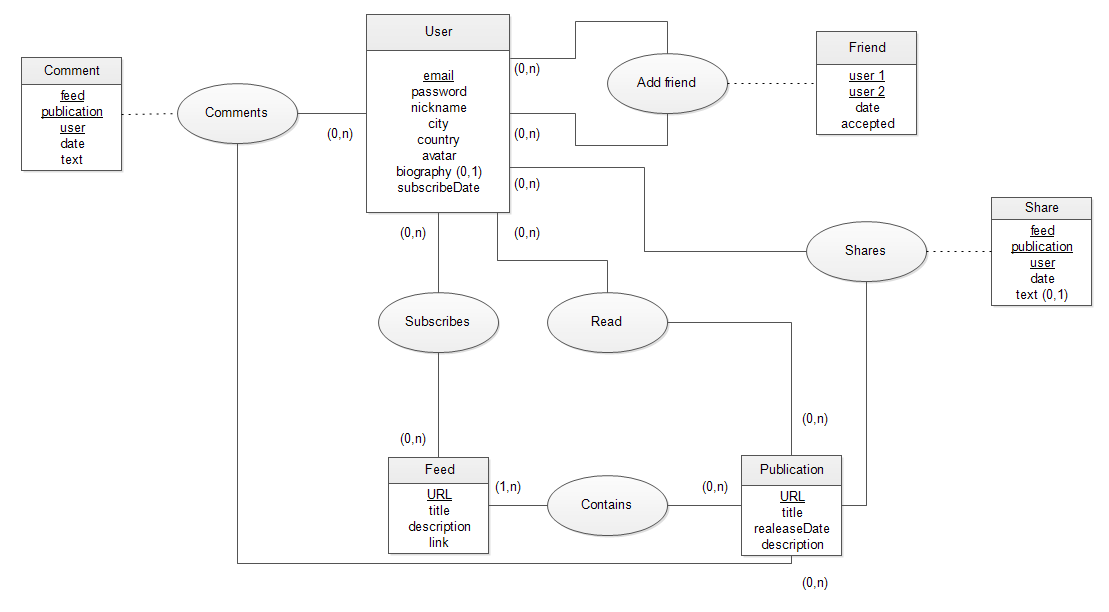
\includegraphics[width = \textwidth]{dea.png}
	\caption{Nous avons ici la modélisation entités-relations du projet.}
	\end{figure}

    \section{Contraintes d'intégrité}
    
    \begin{enumerate}
	\item Lorsqu'un utilisateur A désire effectuer une demande d'amitier il demande a un autre utlisateur B qui peut ou non accepter. Si utilisateur B accepte les utilisateurs sont amis. La demande ne peut être acceptée que par B si elle
	a été demandée par A.
	\item La date d'inscription d'un utilisateur précède les dates de lectures, les dates de commentaires et les dates d'acceptation d'amis.
	\item La date d'une publication précède les dates de lectrue et de commentaires de cette publication.
	\item Les dates de lecture d'un publication précède les dates de commentaires de cette publication.
	\item Les publication d'un flux utilisateur sont exactement les publications que cet utilisateur a partagées.
	\item Un utilisateur ne peut partager ou lire que des publicatipns composant un flux qu'il suit.
	\item Un utlisateur ne peut faire de commentaires que sur une publication partagée par un de ses amis (au moment du commentaire)
	\item Un utilisateur ne peut pas être amis avec lui-même.
	\item L'association d'amitié est bidirectionnelle. Si l'utilisateur A est ami de l'utilisateur B, alors B est ami de l'utilisateur A.
	\item Un utilisateur suit les flux de ses amis.
    \end{enumerate}

    \section{Modélisation relationnelle}

        User (\textbf{email}, password, nickname, city, country, avatar, \textit{biography}, subscription date.)
            \begin{itemize}            
             \item seul le champ \textit{biography} peut être nul
             \item \textit{subscription date} ne peut être dans le futur
             \item \textit{email} doit respecter le format d'e-mail
             \item \textit{city} implique \textit{pays}
            \end{itemize}


        Feed(\textbf{URL}, title, description, \textit{link})
            \begin{itemize}
            \item \textit{URL} doit être une URL valide
	    \end{itemize}
        
        Publication(\textbf{URL}, title, releaseDate, description)
        \begin{itemize}            
            \item \textit{releaseDate} ne peut être dans le futur
        \end{itemize}

        Comment(\textbf{user, publication, feed}, date, text)
        \begin{itemize}
            \item \textit{user} référence \textit{User.email}
            \item \textit{publication} référence \textit{Publication.URL}
            \item \textit{feed} référence \textit{Feed.URL}
            \item \textit{date} ne peut être dans le futur
        \end{itemize}
        
        Friendship(\textbf{user\_1, user\_2}, accepted, date)
        \begin{itemize}            
            \item \textit{user\_1} référence \textit{User.email}
            \item \textit{user\_2} référence \textit{User.email}
            \item \textit{date} ne peut être dans le futur
        \end{itemize}

        Subscribes(\textbf{user, feed}, date)
        \begin{itemize}            
            \item \textit{user} référence \textit{User.email}
            \item \textit{feed} référence \textit{Feed.URL}
            \item \textit{date} ne peut être dans le futur
        \end{itemize}

        Read(\textbf{user, publication, feed}, date)
        \begin{itemize}            
            \item \textit{user} référence \textit{User.email}
            \item \textit{publication} référence \textit{Publication.URL}
            \item \textit{date} ne peut être dans le futur
        \end{itemize}
            
        Contains(\textbf{feed, publication})
        \begin{itemize}            
            \item \textit{feed} référence \textit{Feed.URL}
            \item \textit{publication} référence \textit{Publication.URL}
        \end{itemize}
            
        Share(\textbf{user, publication, feed}, date, text)
        \begin{itemize}
			\item seul le champ \textit{text} peut être nul
            \item \textit{user} référence \textit{User.email}
            \item \textit{publication} référence \textit{Publication.URL}
            \item \textit{feed} référence \textit{Feed.URL}
            \item \textit{date} ne peut être dans le futur
        \end{itemize}
		
\section{Hypothèse}
\begin{itemize}
\item Dans Friendship, user1 est celui qui a fait la demande d'ami et user2 celui qui la recoit.
\item Dans Friendship, une requete avec le flag accepted à 0 est en attente de validation, à 1 elle est validée et si elle est refusé, elle supprimé de la table.
\item Dans Friendship, si accepted vaut 0 alors le champ date vaut celle de la demande, s'il est à 1 alors le champs date représente la date d'ajout en amis.
\item Dans la table Contain, il peut y avoir plusieur référence vers une même publication car cette derniere peut se trouver dans des fluxs personnels en plus de celui du rss de base.
\item Un commentaire ne doit etre affiché que sur certains fluxs. En effet, l'utilisateur ne peut écrire un commentaire uniquement lorsqu'il l'a partagée ou si elle lui a été partagée. Comme il ne peut y avoir qu'un commentaire par publication d'un flux, ces trois éléments sont suffisants pour identifier un commentaire.
\end{itemize}
\section{Choix d'implémentation}
\subsection{Language}
\subsection{Librairie graphique}
		
\section{Instructions d'installation}

Comme il était au départ demandé de pouvoir parser un fichier XML pour peuplé la base de donnée, nous avons créer un générateur de de fichier XML, cependant ce dernier ne crée pas de commentaire de "read" sur des "share", pour la base de donnée peuplée, nous avons utiliser ce générateur et nous avons ajouté manuellement quelque commentaire sur le flux personnel de l'utilisateur Gothdor@gmail.com, dès lors nous vous conseillons de vous connecter avec celui ci.
		
\section{Scénario de démonstration}
\begin{itemize}
\item Creation d'un compte A
\item Connexion de A
\item Ajout d'un flux
\item Ouvrir une publication
\item Passer en mode lu
\item Envoyer une demande d'amis à B
\item Partager une publication
\item Connexion B
\item Accepter A
\item Commenter publication de A
\item Retour compte A, ajouter un deuxième flux
\item Passer en mode toute les publications
\item Modifier son avatar
\item Rechercher un ami et montrer les requètes
\item Rechercher un flux et montrer les requètes
\end{itemize}
		
\section{Requêtes}
\subsection{Requête 1}
Tous les utilisateurs qui ont au plus 2 amis.
\subsubsection{SQL}
\begin{lstlisting}
SELECT * FROM user u
LEFT OUTER JOIN friendship f
ON
(
f.user1_email = u.email
OR
f.user2_email = u.email
)
GROUP BY u.email
HAVING COUNT(u.email) < 3
\end{lstlisting}
\subsubsection{Algèbre relationnel}
\begin{center}
\begin{tabular}{lll}
$Request$		& $\leftarrow$ & $ user\sqsupset\Join_{email=user1\_email \vee email=user2\_email}( friendship)$\\
$Request\_Accepted$	& $\leftarrow$ & $ \sigma_{accepted=TRUE}\ (Request)$\\
$Result$		& $\leftarrow$ & $ \pi_* (email\ \sigma_{COUNT(email)\ <\ 3}\ (Request_Accepted) )$ 
\end{tabular}
\end{center}

\subsubsection{Calcul relationnel tuple}
Définissons le prédicat \emph{Friends(user1, user2)} comme étant:
\\
      $Friends(u_1, u_2):\ \exists\ d\ (Friendship(d)\ \wedge $\\
      $(d.user_1\_email\ =\ u_1.email\ \vee\ d.user_2\_email\ =\ u_2.email)\ \wedge $\\
      $(d.user_2\_email\ =\ u_1.email\ \vee\ d.user_1\_email\ =\ u_2.email)\ \wedge $\\
      $d.accepted\ =\ 1$

La requête devient alors:

       $u | User(u) \wedge$ \\
       $\exists friend_1 ((User(friend_1) \wedge Friends(u, friend_1)) \rightarrow$ \\
       $\exists friend_2 ((User(friend_2) \wedge friend_1 \neq friend_2 \wedge Friends(u, friend_2)) \rightarrow$ \\
       $\nexists friend_3 ((User(friend_3) \wedge friend_1 \neq friend_2 \neq friend_3 \wedge Friends(u, friend_3)))))$
\clearpage
\subsection{Requête 2}
La liste des flux auxquels a souscrit au moins un utilisateur qui a souscrit à au moins deux flux auxquel X
a souscrit.
\subsubsection{SQL}
\begin{lstlisting}
SELECT * FROM feed f
INNER JOIN feedsubscription c ON c.feed_url = f.url
INNER JOIN 
  (
  SELECT b.user_email FROM feedsubscription b 
  INNER JOIN 
    (SELECT feed_url FROM feedsubscription WHERE user_email = <user>.email) a
  ON a.feed_url = b.feed_url 
  GROUP BY b.user_email
  HAVING COUNT(b.user_email) > 1
  ) d
ON d.user_email = c.user_email
GROUP BY c.feed_url
\end{lstlisting}
\subsubsection{Algèbre relationnel}
\begin{center}
\begin{tabular}{lll}
$a$		& $\leftarrow$ & $ \pi_{feed\_url}\ (\sigma_{user\_email=<user>.email}\ (feedsubscription)$\\
$b$		& $\leftarrow$ & $ \pi_{user\_email, feed\_url}\ (feedsubscription)$\\
$b\_a\_join$	& $\leftarrow$ & $ b \Join_{a.feed\_url=b.feed\_url}\ (a)$\\
$d$		& $\leftarrow$ & $ \pi_{b.user\_email}\ (b.user\_email\ \sigma_{COUNT(b.user\_email)\ >\ 1} (b\_a\_join))$\\
$c$		& $\leftarrow$ & $ feedsubscription \Join_{feed\_url=url}\ (f)$\\
$c\_d\_join$	& $\leftarrow$ & $ c \Join_{c.user\_email=d.user\_email} (d)$\\
$Result$	& $\leftarrow$ & $ \pi_*\ (c.feed\_url\ c\_d\_join)$
\end{tabular}
\end{center}
\includegraphics[width=\textwidth]{}

\subsubsection{Calcul relationnel tuple}
\clearpage
\subsection{Requête 3}
La liste des flux auxquels X a souscrit, auxquels aucun de ses amis n’a souscrit et duquel il n’a partagé
aucune publication.
\subsubsection{SQL}

\begin{lstlisting}
SELECT * FROM feed f
INNER JOIN feedsubscription fs1 
  ON 
  fs1.feed_url=f.url AND fs1.user_email = <user>.email
WHERE NOT EXISTS 
  (
  SELECT c1.feed_url FROM contain c1
    INNER JOIN contain c2 
      ON 
      c2.publication_url = c1.publication_url
      AND 
      c2.feed_url = "feed://" + <user>.email
  WHERE c1.feed_url=f.url 
  )
AND NOT EXISTS 
  (
  SELECT fs2.feed_url FROM feedsubscription fs2
    INNER JOIN friendship fr 
    ON 
      (
	fr.user1_email = fs2.user_email
	AND
	fr.user2_email = <user>.email
      )
      OR 
      (
	fr.user2_email = fs2.user_email
	AND
	fr.user1_email = <user>.email
      )
      AND 
	accepted = TRUE
   )
WHERE fs2.feed_url = f.url"

\end{lstlisting}
\subsubsection{Algèbre relationnel}
\begin{center}
\begin{tabular}{lll}
$Shared\_Feeds$ & $\leftarrow$ & $contain \Join_{publication\_url\_1=publication\_url\_2 \wedge feed\_url\_2 = {user.email}}\ (contain)$\\
$Shared\_Feed\_URL$ & $\leftarrow$ & $\pi_{feed_url} \sigma_{feed\_url\_2=url}\ (Shared\_Feeds)$\\
$Friend\_Feeds$ & $\leftarrow$ & $feedsubscription \Join_{((user1\_email=email \wedge user2\_email={user.email}) }$\\
&&$_{\vee (user2\_email=email \wedge user2\_email=[user.email]))} $\\
&&$_{\wedge accepted=TRUE}\ (friendship)$\\
$Friend\_Feed\_URL$ & $\leftarrow$ & $\pi_{feed\_url} \sigma_{feed\_url=url}\ (Friend\_Feeds)$\\
$User\_Feed$ & $\leftarrow$ & $feed \Join_{feed\_url=url \wedge user\_ema1l={user.email}}\ (feedsubscription)$\\
$Result$ & $\leftarrow$ & $(User\_Feed - Shared\_Feed\_URL) - Friend\_Subscribed\_URL$
\end{tabular}
\end{center}

\subsubsection{Calcul relationnel tuple}

\begin{equation*}
 \begin{split}
  \{\ f |\ feed(f)\ \wedge\ \\
  &\quad (\ \exists\ s\ (feedsubscription(s)\ \wedge\ (\ s.feed\_url\ =\ f.url\ \wedge\ s.user\_email\ =\ <\text{user}>.email\ ))\   \wedge \\
  &\quad \quad(\nexists\ c\ (contain(c)\ \wedge\ \exists\ d\ (contain(d)\ \wedge\ d.publication\_url = c.publication\_url\ \wedge\ \\
  &\qquad \qquad d.feed\_url = \text{"feed:// + "}<\text{user}>.email) )\ \wedge \\
  &\quad (\nexists\ e\ (feedsubscription(e)\ \wedge\ \exists\ fs\ (friendship(fs)\ \wedge\ \\
  &\qquad \qquad ((fs.user1\_email\ =\ e.user\_email\ \wedge\ fs.user2\_email\ =\ <\text{user}>.email)\\
  &\qquad \qquad \vee\\
  &\qquad \qquad (fs.user2\_email\ =\ e.user\_email\ \wedge\ fs.user1\_email\ =\ <\text{user}>.email))\\
  &\qquad \qquad \wedge\\
  &\qquad \qquad (fs.accepted\ =\ 1))))\ \wedge \\
  &\quad (e.feed\_url = f.url)
  \end{split}
\end{equation*}

\subsection{Requête 4}
La liste des utilisateurs qui ont partagé au moins 3 publications que X a partagé.
\subsubsection{SQL}
\begin{lstlisting}
SELECT * FROM user u
INNER JOIN sharedpublication s ON s.user_email = u.email
INNER JOIN 
  (
  SELECT publication_url FROM sharedpublication 
  WHERE user_email = <user>.email
  ) a
ON s.publication_url = a.publication_url
GROUP BY s.user_email
HAVING COUNT(s.user_email) > 2
\end{lstlisting}
\subsubsection{Algèbre relationnelle}
\begin{center}
\begin{tabular}{lll}
$a$		& $\leftarrow$ & $\pi_{publication\_url}\ (\ \sigma_{user\_email=<user>.email}\ (sharedpublication))$\\
$s$		& $\leftarrow$ & $user \Join_{email = user\_email} (sharedpublication)$\\
$a\_s\_join$	& $\leftarrow$ & $a \Join_{a.publication\_url=s.publication_url} (s)$\\
$Result$	& $\leftarrow$ & $\pi_*\ (s.user\_email\ \sigma_{COUNT(s.user_email) > 2} (a\_s\_join))$
\end{tabular}
\end{center}

\subsubsection{Calcul relationnel tuple}
Définissons le prédicat \emph{ResharedPublication(user1, user2)} comme étant:
\\
      $ResharedPublication(u_1, u_2):\ $\\
	  $\exists\ s\ (Sharedpublication(publication\_url)\ \wedge s.user\_email\ =\ u_1.email)\ \wedge $\\
	  $\exists\ a\ (Sharedpublication(publication\_url)\ \wedge s.user\_email\ =\ u_2.email)\ \wedge $\\
	  $a.publication\_url = s.publication\_url$

La requête devient alors:

       $u\ |\ User(u) \wedge$ \\
       $\exists \ publication_1 \ ((Sharedpublication(publication_1) \ \wedge \ ResharedPublication(u, \ <user>)) \ \wedge$ \\
       $\exists \ publication_2 \ (Sharedpublication(publication_2) \ \wedge \ publication_1 \ \neq \ publication_2 \ \wedge \ ResharedPublication(u, \ <user>)) \ \wedge$ \\
       $\exists \ publication_3 \ (Sharedpublication(publication_3) \ \wedge \ publication_1 \ \neq \ publication_2 \ \neq \ publication_3 \ \wedge  \ ResharedPublication(u, \ <user>)))$
\clearpage
\subsection{Requête 5}
La liste des flux auquel un utilisateur est inscrit avec le nombre de publications lues, le nombre de publications
partagées, le pourcentage de ces dernières par rapport aux premières, cela pour les 30 derniers jours et ordonnée
par le nombre de publications partagées.
\subsubsection{SQL}
\begin{lstlisting}
SELECT f.url, f.title, f.description, f.link, f.image, 
(
  SELECT COUNT(*) FROM readstatus rs 
  WHERE 
    rs.feed_url = f.url
  AND 
    rs.user_email = fs2.user_email
  AND 
    TO_DAYS(NOW())-TO_DAYS(rs.date) < 30
)
AS nread,
(
  SELECT COUNT(*) FROM sharedpublication sp
  INNER JOIN feedsubscription fs 
    ON 
      sp.user_email = fs.user_email
  INNER JOIN contain c 
    ON 
	fs.feed_url = c.feed_url
      AND 
	sp.publication_url = c.publication_url
  WHERE 
    c.feed_url = f.url
  AND 
    sp.user_email = fs2.user_email
  AND 
    TO_DAYS(NOW())-TO_DAYS(sp.sharedDate) < 30
) 
AS nshared,
( 
  SELECT nshared/nread 
)
AS ratio 
FROM feed f
INNER JOIN feedsubscription fs2 
ON 
  fs2.feed_url = f.url
WHERE 
  fs2.user_email = <user>.email 
GROUP BY 
  f.url 
ORDER BY nshared
\end{lstlisting}
\clearpage
\subsection{Requête 6}
La liste des amis d’un utilisateur avec pour chacun le nombre de publications lues par jour et le nombre
d’amis, ordonnée par la moyenne des lectures par jour depuis la date d’inscription de cet ami

\subsubsection{SQL}
\begin{lstlisting}
SELECT u.*,
(
  SELECT COUNT(*) FROM readstatus rs 
  WHERE 
  rs.user_email = u.email)/(TO_DAYS(NOW())-TO_DAYS(u.joinedDate)
) 
AS mread,
(
  SELECT COUNT(u2.email) FROM user u2
  INNER JOIN friendship f2 
  ON 
      f2.user1_email = u2.email 
    OR 
      f2.user2_email = u2.email
  WHERE 
  u2.email = u.email 
  GROUP BY u2.email
) 
AS nfriend
FROM user u
INNER JOIN friendship f 
ON 
    f.user1_email = u.email 
  OR 
    f.user2_email = u.email
WHERE 
  (
    f.user1_email = <user>.email 
  AND 
    u.email <> f.user1_email
  ) 
OR 
  (
    f.user2_email = <user>.email 
  AND 
    u.email <> f.user2_email
  )
ORDER BY mread
\end{lstlisting}
		
\section{Script SQL DDL}
\begin{lstlisting}

SET SQL_MODE = "NO_AUTO_VALUE_ON_ZERO";
SET time_zone = "+00:00";


/*!40101 SET @OLD_CHARACTER_SET_CLIENT=@@CHARACTER_SET_CLIENT */;
/*!40101 SET @OLD_CHARACTER_SET_RESULTS=@@CHARACTER_SET_RESULTS */;
/*!40101 SET @OLD_COLLATION_CONNECTION=@@COLLATION_CONNECTION */;
/*!40101 SET NAMES utf8 */;

--
-- Bdd :  `rssreader`
--
CREATE DATABASE IF NOT EXISTS `rssreader` DEFAULT CHARACTER SET utf8 COLLATE utf8_bin;
USE `rssreader`;

-- --------------------------------------------------------

--
-- Structure de la table `comment`
--

CREATE TABLE IF NOT EXISTS `comment` (
  `feed_url` varchar(200) COLLATE utf8_bin NOT NULL,
  `publication_url` varchar(200) COLLATE utf8_bin NOT NULL,
  `user_email` varchar(200) COLLATE utf8_bin NOT NULL,
  `date` date NOT NULL,
  `text` text COLLATE utf8_bin NOT NULL,
  PRIMARY KEY (`feed_url`,`publication_url`,`user_email`)
) ENGINE=InnoDB DEFAULT CHARSET=utf8 COLLATE=utf8_bin;

-- --------------------------------------------------------

--
-- Structure de la table `contain`
--

CREATE TABLE IF NOT EXISTS `contain` (
  `feed_url` varchar(200) COLLATE utf8_bin NOT NULL,
  `publication_url` varchar(200) COLLATE utf8_bin NOT NULL,
  PRIMARY KEY (`feed_url`,`publication_url`)
) ENGINE=InnoDB DEFAULT CHARSET=utf8 COLLATE=utf8_bin;

-- --------------------------------------------------------

--
-- Structure de la table `feed`
--

CREATE TABLE IF NOT EXISTS `feed` (
  `url` varchar(200) COLLATE utf8_bin NOT NULL,
  `title` varchar(200) COLLATE utf8_bin NOT NULL,
  `link` varchar(200) COLLATE utf8_bin NOT NULL,
  `description` text COLLATE utf8_bin NOT NULL,
  `image` varchar(200) COLLATE utf8_bin DEFAULT NULL,
  PRIMARY KEY (`url`)
) ENGINE=InnoDB DEFAULT CHARSET=utf8 COLLATE=utf8_bin;

-- --------------------------------------------------------

--
-- Structure de la table `feedsubscription`
--

CREATE TABLE IF NOT EXISTS `feedsubscription` (
  `user_email` varchar(200) COLLATE utf8_bin NOT NULL,
  `feed_url` varchar(200) COLLATE utf8_bin NOT NULL,
  `subscribedDate` date NOT NULL,
  PRIMARY KEY (`user_email`,`feed_url`)
) ENGINE=InnoDB DEFAULT CHARSET=utf8 COLLATE=utf8_bin;

-- --------------------------------------------------------

--
-- Structure de la table `friendship`
--

CREATE TABLE IF NOT EXISTS `friendship` (
  `user1_email` varchar(200) COLLATE utf8_bin NOT NULL,
  `user2_email` varchar(200) COLLATE utf8_bin NOT NULL,
  `requestDate` date NOT NULL,
  `accepted` tinyint(1) NOT NULL,
  PRIMARY KEY (`user1_email`,`user2_email`)
) ENGINE=InnoDB DEFAULT CHARSET=utf8 COLLATE=utf8_bin;

-- --------------------------------------------------------

--
-- Structure de la table `publication`
--

CREATE TABLE IF NOT EXISTS `publication` (
  `url` varchar(200) COLLATE utf8_bin NOT NULL,
  `title` varchar(200) COLLATE utf8_bin NOT NULL,
  `releaseDate` date NOT NULL,
  `description` text COLLATE utf8_bin NOT NULL,
  `image` varchar(200) COLLATE utf8_bin DEFAULT NULL,
  PRIMARY KEY (`url`)
) ENGINE=InnoDB DEFAULT CHARSET=utf8 COLLATE=utf8_bin;

-- --------------------------------------------------------

--
-- Structure de la table `readstatus`
--

CREATE TABLE IF NOT EXISTS `readstatus` (
  `user_email` varchar(200) COLLATE utf8_bin NOT NULL,
  `publication_url` varchar(200) COLLATE utf8_bin NOT NULL,
  `feed_url` varchar(200) COLLATE utf8_bin NOT NULL,
  `date` date NOT NULL,
  PRIMARY KEY (`user_email`,`publication_url`,`feed_url`)
) ENGINE=InnoDB DEFAULT CHARSET=utf8 COLLATE=utf8_bin;

-- --------------------------------------------------------

--
-- Structure de la table `sharedpublication`
--

CREATE TABLE IF NOT EXISTS `sharedpublication` (
  `user_email` varchar(200) COLLATE utf8_bin NOT NULL,
  `publication_url` varchar(200) COLLATE utf8_bin NOT NULL,
  `sharedDate` date NOT NULL,
  `text` text COLLATE utf8_bin,
  PRIMARY KEY (`user_email`,`publication_url`)
) ENGINE=InnoDB DEFAULT CHARSET=utf8 COLLATE=utf8_bin;

-- --------------------------------------------------------

--
-- Structure de la table `user`
--

CREATE TABLE IF NOT EXISTS `user` (
  `email` varchar(200) COLLATE utf8_bin NOT NULL,
  `nickname` varchar(100) COLLATE utf8_bin NOT NULL,
  `password` varchar(100) COLLATE utf8_bin NOT NULL,
  `country` varchar(100) COLLATE utf8_bin NOT NULL,
  `city` varchar(100) COLLATE utf8_bin NOT NULL,
  `avatar` varchar(200) COLLATE utf8_bin NOT NULL,
  `biography` text COLLATE utf8_bin,
  `joinedDate` date NOT NULL,
  PRIMARY KEY (`email`)
) ENGINE=InnoDB DEFAULT CHARSET=utf8 COLLATE=utf8_bin;

/*!40101 SET CHARACTER_SET_CLIENT=@OLD_CHARACTER_SET_CLIENT */;
/*!40101 SET CHARACTER_SET_RESULTS=@OLD_CHARACTER_SET_RESULTS */;
/*!40101 SET COLLATION_CONNECTION=@OLD_COLLATION_CONNECTION */;

\end{lstlisting}

\end{document}
